%!TEX program = xelatex
%!TEX encoding = UTF-8 Unicode

\documentclass[10pt, twocolumn]{article}
\usepackage[top=1in, bottom=1in, left=1in, right=1in]{geometry}

% ----- ADDITIONAL PACKAGES -----
\usepackage{fontspec,xltxtra,xunicode}
\usepackage[usenames,dvipsnames]{color}
\usepackage[bookmarks, colorlinks, breaklinks, 
  pdfauthor={Yue Wu},
  pdfcreator={xelatex}
]{hyperref}
\usepackage{amsmath}
\usepackage{amsfonts}
\usepackage{paralist}

% ----- SETTINGS -----
\setcounter{secnumdepth}{0}
\linespread{1.15}
\setlength\parindent{0pt}
\setlength\parskip{1ex plus 0.2ex minus 0.1ex}
\setlength\emergencystretch{3em}
\hypersetup{linkcolor=blue, citecolor=blue, filecolor=black, urlcolor=MidnightBlue}

% ----- DOCUMENT -----
\begin{document}
\pagestyle{myheadings}
\markright{Yue Wu}

\section*{Basic Statistics} \vspace*{-1em}
\begin{itemize}
\item Conditional Prob: $P(A|B)=P(A\cap B)/P(B)$
\item Independent $\Longleftrightarrow P(A\cap B)=P(A)P(B)$
% \begin{table}[h] \centering
% \begin{tabular}{|c|c|c|} \hline
% RV $X$    & Prob. $f(x)$     & CDF $F(x)$               \\ \hline
% Disc(pmf) & $\sum_xf(x)=1$   & $\sum_{y\leq x}f(y)$     \\ \hline
% Cont(pdf) & $\int_xf(x)dx=1$ & $\int_{-\infty}^xf(y)dy$ \\ \hline
% \end{tabular}
% \end{table}
% \item $X$ is continuous RV $\Rightarrow F(X) \sim \text{Unif}(0,1)$ 
% \item $E[(X-\mu)^n]$ is the $n$th \emph{central moment} of $X$
% \item $M_X(t)\equiv E[e^{tX}]$: \emph{moment generating function}
% \item Under certain technical conditions, 
% \[ E[X^k]=\frac{d^k}{dt^k}M_X(t)|_{t=0},\ k=1,2,\dots \]
\item $Var[X]=E[X^2]-E^2[X]$
\item $E[aX+b]=aE[X]+b$, $V[aX+b]=a^2V[X]$
\item Joint CDF: $F(x,y)\equiv P(X\leq x, Y\leq y),\ \forall x,y$
\item Joint PDF: $f(x,y)\equiv \frac{\partial^2}{\partial x\partial y}F(x,y)$
\item Marginal CDF: $F_X(x)=\int F(x,y)dy$
% \item \emph{Independent} $\Longleftrightarrow f(x,y)=f_X(x)f_Y(y) \Longleftrightarrow f(x,y)=a(x)b(y)$ and domains are independent % $\Longleftrightarrow f(y|x)=f_Y(y)$
\item Conditional PDF: $f(y|x)\equiv f(x,y)/f_X(x)$
% \item $E[Y|X=x]=\int yf(y|x)dy$, $E[E(Y|X)]=E[Y]$
\item $E[XY]=\iint xyf(x,y)dxdy$
\item $Cov(X,Y)=E[XY]-E[X]E[Y]$ \\
$Cov(aX,bY)=abCov(X,Y)$ \\
$Cov(X\pm Y,Z)=Cov(X,Z)\pm Cov(Y,Z)$
\item $Corr(X,Y)\equiv Cov(X,Y)/\sqrt{V(X)V(Y)}$ \\ 
$Corr(aX,bY)=Corr(X,Y)$
\item Independent $\Rightarrow Cov(X,Y)=0$
\item $Var(X\pm Y)=Var(X)+Var(Y)\pm 2Cov(X,Y)$
\item Bayes' Formula: 
\[ \text{Pr}(E_i|O_j)= \frac{\text{Pr}(O_j|E_i)\text{Pr}(E_i)}{\sum\text{Pr}(O_j|E_i)\text{Pr}(E_i)} \]
\end{itemize}

\section*{Probability Distributions} \vspace*{-1em}
\begin{itemize}
\item $X\sim \text{Bernoulli}(p)$:
\[ f(x) = \left\{ 
  \begin{array}{c l}
    p & \quad \text{if $x=1$}\\
    1-p & \quad \text{if $x=0$}
  \end{array} \right.\]
$E[X]=p$, $Var(X)=p(1-p)$
\item $X\sim \text{Binomial}(n,p)$: \\
(\# of successes in $n$ $\text{Bern}(p)$ trials)
\[ f(x)={n \choose x}p^x(1-p)^{n-x} \]
$E[X]=np$, $Var(X)=np(1-p)$
\item $X\sim \text{Geometric}(p)$: \\
(\# of $\text{Bern}(p)$ trials until a success occurs)
\[ f(x) = (1-p)^{x-1}p \]
$E[X]=1/p$, $Var(X)=(1-p)/p^2$
% \item $X\sim \text{NegBin}(r,p)$: the sum of $r$ iid $\text{Geom}(p)$
% \[ f(x)={x-1 \choose r-1}(1-p)^{x-r}p^r,\ x=r,r+1,\dots \]
% $E(X)=r/p$, $Var(X)=r(1-p)/p^2$
\item $X\sim \text{Poisson}(\lambda)$: 
\[ f(x) = \frac{e^{-\lambda}\lambda ^x}{x!},\ x=0,1,\dots \]
$E[x]=\lambda=Var(X)$
\item $X\sim \text{Uniform}(a,b)$: 
\[ f(x)=\frac{1}{b-a},\ E[X]=\frac{a+b}{2},\ V(X)=\frac{(b-a)^2}{12} \]
\item $X\sim \text{Exponential}(\lambda)$: time between Poi events
\[ f(x)=\lambda e^{-\lambda x},\ F(x)=1-e^{-\lambda x}, \]
$E[X]=1/\lambda$, $Var(X)=1/\lambda^2$. And 
\[ P(X>s+t|X>s)=P(X>t) \]
% \emph{memoryless property} $\Uparrow$
\item $X\sim \text{Erlang}(k, \lambda)$: the sum of $k$ $\text{Exp}(\lambda)$
\[ f(x)=\frac{\lambda^kx^{k-1}e^{-\lambda x}}{(k-1)!},\ for\ x,\lambda\geq0 \]
\[ F(x)=1-\sum_{n=0}^{k-1}\frac{e^{-\lambda x}(\lambda x)^n}{n!} \]
$E(X)=k/\lambda$, $Var(X)=k/\lambda^2$
% \item $X\sim \text{Beta}(a,b)$: \\ 
% \[ E(X)=\frac{a}{a+b},\ V(X)=\frac{ab}{(a+b)^2(a+b+1)} \]
% \item $X\sim \text{Gamma}(\alpha,\lambda)$: 
% \[ E[X]=\alpha/\lambda,\ Var(X)=\alpha/\lambda^2 \]
\item $X\sim \text{Triangular}(a,b,c)$: $E(X)=(a+b+c)/3$
\item $X\sim \text{Normal}(\mu,\sigma^2)$: 
\[ f(x) = \frac{1}{\sqrt{2\pi\sigma^2}}\text{exp}\left[-\frac{(x-\mu)^2}{2\sigma^2}\right],\ x\in\mathbb{R} \]
$E[X]=\mu$, $V[X]=\sigma^2$, $M_X(t)=exp[\mu t+\frac{1}{2}\sigma^2t^2]$
% \item $X\sim \text{LogNormal}(\mu,\sigma^2)$:
% \[ f(x) = \frac{1}{x\sqrt{2\pi\sigma^2}}\text{exp}\left[-\frac{(\ln x-\mu)^2}{2\sigma^2}\right% ],\ x\in\mathbb{R}^+ \]
% $E[X]=e^{\mu+\sigma^2/2}$, $V[X]=(e^{\sigma^2}-1)e^{2\mu+\sigma^2}$
\item \emph{Law of Large Numbers} (special case): 
\[ X_1,\dots,X_n \text{ are iid Nor} \Rightarrow \bar{X}_n\sim \text{Nor}(\mu,\sigma^2/n) \]
\item \emph{Central Limit Theorem}: If $X_1,\dots,X_n\stackrel{iid}{\sim}f(x)$, 
\[ Z_n\equiv \frac{\bar{X}_n-\mu}{\sigma/\sqrt{n}}\stackrel{d}{\longrightarrow}\text{Nor}(0,1) \]
% \item $100(1-\alpha)\%$ \emph{Confidence Intervals}: 
% \[ \mu\in[\bar{X}_n-z_{\alpha/2}\sqrt{\frac{\sigma^2}{n}},\bar{X}_n+z_{\alpha/2}\sqrt{\frac{\sigma^2}{n}}] \text{ or}\]
% \[ \mu\in[\bar{X}_n-t_{\alpha/2,n-1}\sqrt{\frac{S^2}{n}},\bar{X}_n+t_{\alpha/2,n-1}\sqrt{\frac{S^2}{n}}] \]
% in which, $S^2=\frac{1}{n-1}\sum_{i=1}^n(X_i-\bar{X}_n)^2$
\end{itemize}

\section*{Input Modeling} \vspace*{-1em}
Represent the uncertainty in a stochastic simulation. \vspace*{-3em}
\begin{itemize}
\item Fundamental Requirements: 
\begin{inparaenum}
  \item capable of representing the physical realities of the process; 
  \item easily tuned to the situation on hand; and 
  \item amenable to random variate generation. 
\end{inparaenum}
\item Input Modeling with Data: 
\begin{inparaenum}
  \item select one or more candidate distribution, based on physical characteristics of the process and graphical examination of the data; 
  \item fit the distribution with data; 
  \item check the fit to the data via tests and graphical analysis; and 
  \item if the distribution does not fit, select another candidate and go to 2, or use an empirical distribution. 
\end{inparaenum}
\item Physical Basis for Distributions: 
\begin{inparaenum}
  \item \textbf{Binomial}: \# of successes in $n$ iid $\text{Bernoulli}(p)$ trials; 
  \item \textbf{Negative Binomial}: \# of trials required to achieve k ``successes'' (the sum of $k$ iid $\text{Geom}(p)$); 
  \item \textbf{Poisson}: \# of independent events that occur in a fixed amount of time or space; 
  \item \textbf{Normal}: the distribution of a process that can be thought of as the sum of a number of component processes; 
  \item \textbf{Lognormal}: the distribution of a process that can be thought of as the product of a number of component processes; 
  \item \textbf{Exponential}: the time between independent events, or a process time which is memoryless; 
  \item \textbf{Erlang}: the sum of k identical exponential random variables; 
  \item \textbf{Gamma}: an extremely flexible distribution used to model nonnegative random variables; 
  \item \textbf{Beta}: an extremely flexible distribution used to model bounded (fixed upper and lower limits) random variables; 
  \item \textbf{Weibull}: the time to failure for components, can model increasing or decreasing failure rate hazard; 
  \item \textbf{Uniform}: models complete uncertainty, since all outcomes are equally likely; 
  \item \textbf{Triangular}: models a process when only the minimum, most likely and maximum values of the distribution are known; 
  \item \textbf{Empirical}: reuses the data themselves by making each observed value equally likely, can be interpolated to obtain a continuous distribution.
\end{inparaenum}
\item Common Methods for Fitting: maximum likelihood, method of moments, and least squares. (While the method matters, the variability in the data often overwhelms the differences in the estimators.) 
\item Ways to Check Fit: $\chi^2$, K-S, Anderson-Darling tests; density-histogram, and q-q plots. 
\item p-value: Type I error level (significance) at which we would just reject $H_0$ for the
given data. (less likely to reject $H_0$ at larger p-value)
\item q-q Plot: displays the sorted data ($Y_1 \leq Y_2 \leq \dots \leq Y_n$) vs $F^{-1}((j-1/2)/n), j=1,2,\dots,n$. \textbf{Features}: 
\begin{inparaenum}
  \item does not depend on how the data are grouped; 
  \item better than density-histogram when the number of data points is small; and
  \item deviations from a straight line show where the distribution does not match (a straight line implies the family of distributions is correct; a $45\textdegree$ line implies correct parameters, a curved line implies a wrong dist'n family). 
\end{inparaenum}
\item $\chi^2$ Test: 
\begin{inparaenum}
  \item a formal comparison of a histogram or line graph with the fitted density or mass function; and
  \item sensitive to how we group the data. 
\end{inparaenum}
\item K-S and A-D Test: 
\begin{inparaenum}
  \item comparison of an empirical distribution function with the distribution function of the hypothesized distribution; 
  \item does not depending on the grouping of data; and 
  \item A-D detects discrepancies in the tails and higher power than K-S test.
\end{inparaenum} 
\item Beware of goodness-of-fit tests because they are unlikely to reject any distribution when you have little data, and are likely to reject every distribution when you have lots of data; Avoid histogram-based summary measures, if possible, when asking the software for its recommendation.
\item Empirical Distribution: 
\begin{inparaenum}
  \item As the sample size goes to infinity, the empirical distribution converges to ``the truth''; 
  \item no assumed distribution need to be selected; and 
  \item only the values we saw can appear again, no tails and nothing in the gaps. 
\end{inparaenum}
\item Interpolated Empirical: to fill in gaps, we linearly interpolate between the sorted data points. 
\item Breakpoints Method: useful for modeling quantities with a large number of possible outcomes. (smallest and largest possible values, most likely value, 1-3 breakpoints)
\item Mean \& Variability Method: ..., also useful for modeling the variability in percentage changes. (mean value, an average percentage variation around that mean, upper and lower limits)
\item Correlations: if data exists, calculate sample correlation; if not, percentage of the time the two inputs move together ($P\%$), then $|\rho|=P/100$.
\end{itemize}

\section*{Inventory Management} \vspace*{-1em}
\begin{itemize}
\item News Vendor Problem: total cost is 
\[ c_p\text{min}\{D,y\} + c_s(y-D)^+ - c_vy \Rightarrow \]
\[ c_pD - \{c_vy + c_p(D-y)^+ - c_s(y-D)^+\} \]
optimal quantity: $F(y^*) \geq (c_p-c_v)/(c_p-c_s)$
\item EOQ with Certain Demand: 
\[ \text{TC}(q) = \frac{KD}{q} + pD + \frac{hq}{2} \Rightarrow 
q^* = \sqrt{\frac{2KD}{h}} \]
\item EOQ with Uncertain Demand (back-ordered): 
\[ K\frac{\text{E}[D]}{q} + h(r-\text{E}[X]+\frac{q}{2}) + c_B\text{E}[B]\frac{\text{E}[D]}{q} \]
\[ q^* = \sqrt{\frac{2\text{E}[D](K+c_B\text{E}[B])}{h}} \]
\[ \text{Pr}(X \geq r^*) = \frac{hq^*}{c_B\text{E}[D]} \]
\item \# of Backorder: $\text{E}[B]=\sigma_XL_{SN}(\frac{r-\mu_X}{\sigma_X})$
\item Safety Stock: $ss = r-\text{E}[X]$
\item Ordering \& Transportation: $p\text{E}[D]+K\text{E}[D]/q$ \\
Pipeline Inventory: $\text{E}[D]ivL$ \\
Facility Inventory: $iv(q/2+ss)+s(q+ss)$ \\
Backordered demand: $c_B\text{E}[B]\text{E}[D]/q$
\item EOQ with Uncertain Demand (loss sales):
\[ K\frac{\text{E}[D]}{q} + h(r-\text{E}[X]+\frac{q}{2}+\text{E}[B]) + c_{LS}\text{E}[B]\frac{\text{E}[D]}{q} \]
\[ q^* = \sqrt{\frac{2\text{E}[D](K+c_{LS}\text{E}[B])}{h}} \]
\[ \text{Pr}(X \geq r^*) = \frac{hq^*}{hq^*+c_{LS}\text{E}[D]} \]
\item Service Level Measure 1: fraction of all demand $D$ that is met on time ($\beta=1-\text{E}[B]/q$).
\item Service Level Measure 2: proportion of cycles in which no shortage occurs ($\alpha=1-\text{Pr}(X>r)$).
\item Standard Normal Loss Function: % $L_{SN}(-c)=c+L_{SN}(c)$
\[ L_{SN}(z) = \varphi(z) - z[1-\Phi(z)], \varphi(z)=\frac{e^{-z^2/2}}{\sqrt{2\pi}} \]
\item $L$ is constant: $D_{R+L} \sim \text{Nor}\{(R+L)\text{E}[D], (R+L)\text{V}[D]\}$; otherwise: $D_{R+L} \sim \text{Nor}\{R\text{E}[D]+\text{E}[L]\text{E}[D], R\text{V}[D]+\text{E}[L]\text{V}[D]+\text{E}^2[D]\text{V}[L]\}$
\item Order Up to Policy (back-ordered): 
\[ p\text{E}[D] + \frac{K+J}{R} + h(S-\text{E}[D_{R+L}]+\frac{1}{2}\text{E}[D_R]) + c_B\frac{\text{E}[B]}{R} \]
\[ \text{EOQ} = \sqrt{\frac{2(K+J)\text{E}[D]}{h}} \]
\[ \text{Pr}(D_{R+L} \geq S) = hR/c_B \]
\item $\text{E}[B] = \sqrt{(R+L)\text{V}[D]}L_{SN}\left(\frac{S-(R+L)\text{E}[D]}{\sqrt{(R+L)\text{V}[D]}}\right)$
\item Find $S$ that $\text{Pr}(D_{R+L}>S)=1-\alpha$: 
\[ S = (R+L)\text{E}[D]+z_{1-\alpha}\sqrt{(R+L)\text{V}[D]} \]
\item Fill Rate: $\text{E}[B]/(R\text{E}[D])=1-\beta$
\item Order Up to Policy (loss sales):
\[ \text{Pr}(D_{R+L} \geq S) = hR/(hR+c_{LS}) \]
\item Ordering \& Transportation: $p\text{E}[D]+K/R$ \\
Pipeline Inventory: $\text{E}[D]ivL$ \\
Facility Inventory: $h(\frac{R\text{E}[D]}{2}+ss)+s(R\text{E}[D]+ss)$ \\
Back-ordered demand: $c_B\text{E}[B]/R$
\item \large{\textbf{Annually Cost $\Rightarrow$ Weekly!}}
\end{itemize}

\section*{Queuing System (A/B/C/K/N)} \vspace*{-1em}
\begin{itemize}
\item A: interarrival time $\lambda$ (M/EXPO, D/DETER, E/ERLANF, G/GENERAL); B: service time $\mu$; C: \# of identical and parallel servers; K: system capacity (buffer + servers); N: population size
\item $X(t)$: \# of customer in system at time $t$; \\
$\pi=\{\pi_0,\pi_1,\dots\}$: probability of $n$ in queue; \\
$\rho=1-\pi_0$: fraction of time that a server is busy; \\
$L=\sum_{i=0}^{\infty}i\pi_i$: \# of customer in the system; \\
$L_q=\sum_{i=1}^{\infty}(i-1)\pi_i$: \# of customer queuing; \\
$W=L/\lambda_{\text{eff}}$: average time in system; \\
$W_q=L_q/\lambda_{\text{eff}}$: average time queuing
\begin{figure}[!h]
\centering
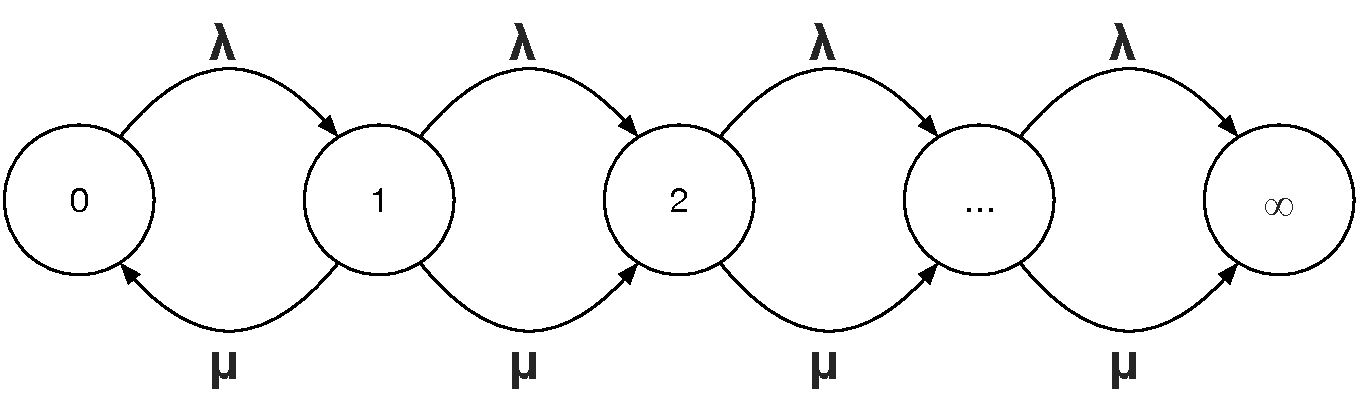
\includegraphics[width=2.5in]{MM1}
\end{figure}
\item M/M/1: (little's law: $L = \lambda_{eff} \times W$) \\
$\pi_n=(\lambda/\mu)^n\pi_0$, $\pi_0 = (\lambda/\mu)^n(1-\lambda/\mu)$ \\
$\rho=1-\pi_0=\lambda/\mu$ \\
$L=\lambda/(\mu-\lambda)$, $L_q=\lambda^2/(\mu^2-\mu\lambda)$ \\
$W=1/(\mu-\lambda)$, $W_q=\lambda/(\mu^2-\mu\lambda)$
\begin{figure}[!h]
\centering
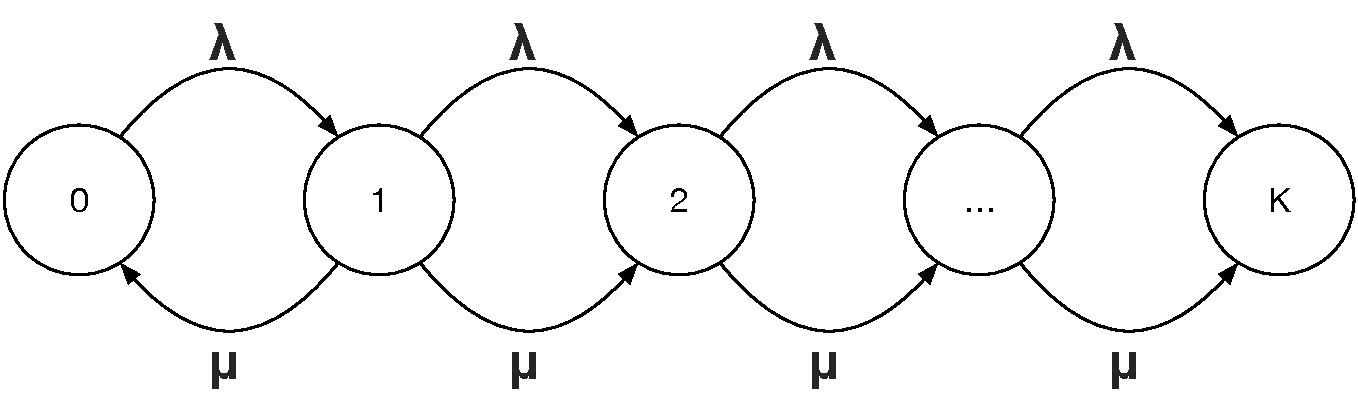
\includegraphics[width=2.5in]{MM1K}
\end{figure}
\item M/M/1/K: $\mu\pi_1=\lambda\pi_0$, $\mu\pi_k=\lambda\pi_{k-1}$ \\
$\lambda\pi_{i-1}+\mu\pi_{i+1}=(\mu+\lambda)\pi_{i},\ (1 \leq i \leq k-1)$
\begin{figure}[!h]
\centering
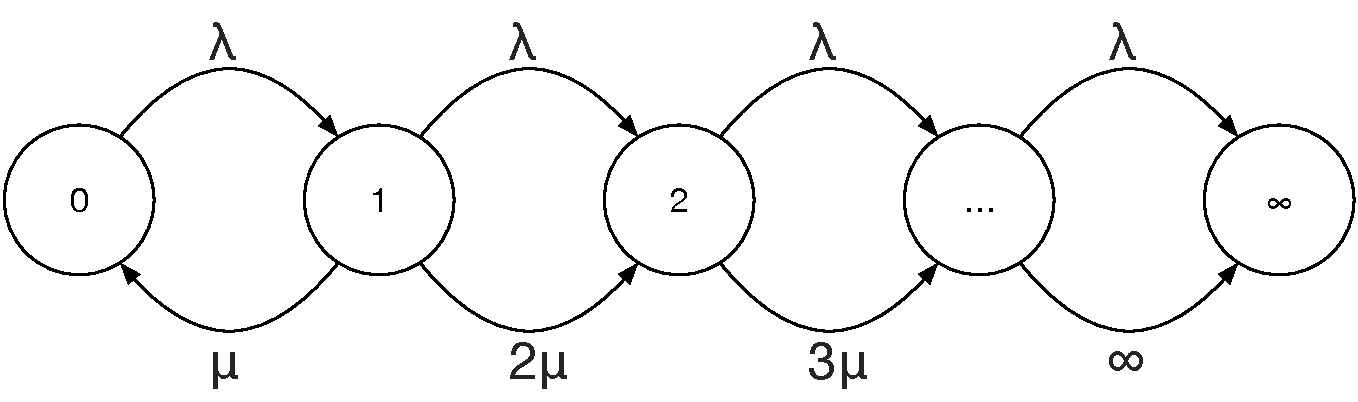
\includegraphics[width=2.5in]{MM8}
\end{figure}
\item M/M/$\infty$: $\pi_0=e^{-\lambda/\mu}$, $\pi_n=e^{-\lambda/\mu}(\lambda/\mu)^n/n!$
\begin{figure}[!h]
\centering
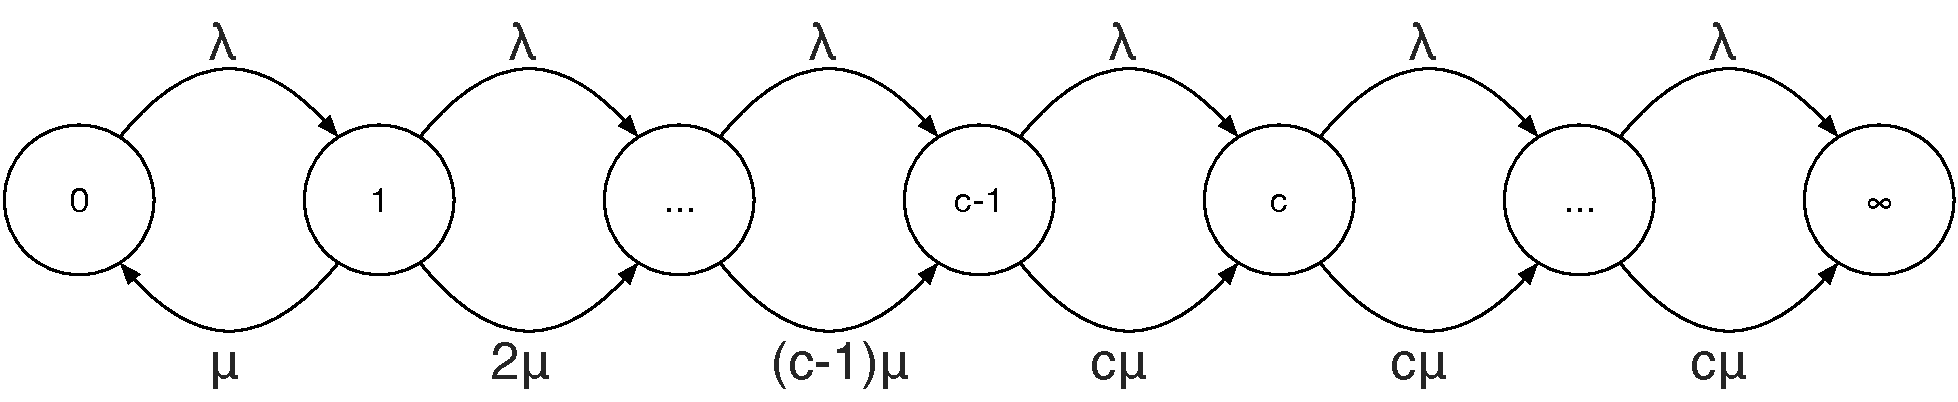
\includegraphics[width=2.5in]{MMC}
\end{figure}
\item M/M/C: $\rho=\lambda/(c\mu)$, $L_q=\sum_{i=1}^{\infty}i\pi_{c+i}$ \\
$W_q=L_q/\lambda$, $W=W_q+1/\mu$
\begin{figure}[!h]
\centering
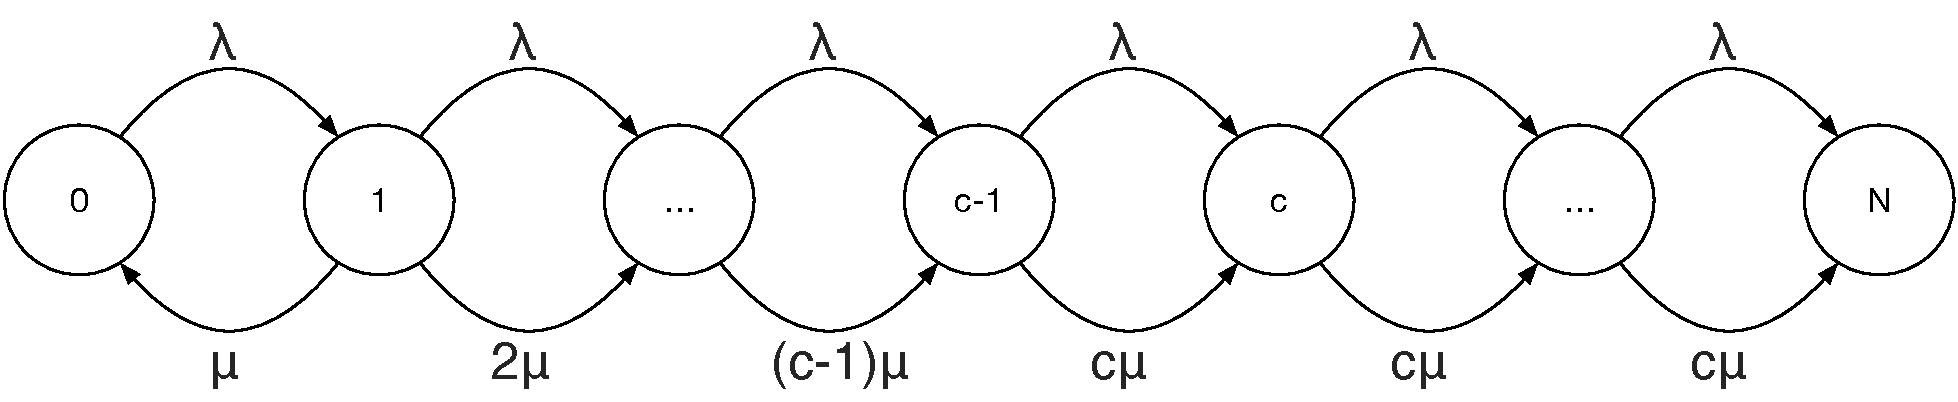
\includegraphics[width=2.5in]{MMCN}
\end{figure}
\item M/M/C/N: $\lambda_{\text{eff}}=\lambda\text{Pr(accept)}$
\item G/G/1: for large $\rho=\lambda/\mu$, $W_q=\frac{1}{\mu}\frac{\rho}{1-\rho}\frac{c_a^2+c_s^2}{2}$ \\ 
$c_a^2=\text{Var}(\text{interarrival time})/\text{E}^2(\text{interarrival time})$ \\
$c_s^2=\text{Var}(\text{service time})/\text{E}^2(\text{service time})$
\item G/G/C: $W_q=(W_q\text{ for M/M/C})\times(1+c_s^2)/2$
\end{itemize}
\end{document}